\section{What the prepared state is made of}
\label{sec:static}

Section~\ref{sec:measured} measured how much entanglement the evolved state carries. What that entanglement means, and what the task costs, depends on a different question: \emph{what is the start state in terms of the eigenstates of $\hat H$?} If it lies on very few of them, the signal $\langle\Op\rangle(t)$ is a short sum of cosines whose frequencies, weights and amplitudes are static quantities of $\hat H$. This section reports the low levels of $\hat H$ at the resonance tilt and the weight of the correlated start on each (no propagation) for $N\le5$, and for $N=6$ in one basis; Table~\ref{tab:static} summarizes it and Table~\ref{tab:start} (Appendix~\ref{app:static}) has every case. The \emph{pair} is the two levels of largest weight, at energies $E_a<E_b$, with $J=(E_b-E_a)/2$ and total weight $B_2$.

\paragraph{What is observed.}
\begin{itemize}[itemsep=0.15em]
\item The start is two eigenstates, the cluster before and after one particle has moved, plus a dressing by soft internal levels whose weight grows with $N$.
\item An exact reflection symmetry removes all other levels from the picture, and the transfer of more than one particle lies far from the pair.
\item Most of the cut entropy of Section~\ref{sec:measured} is present without any tunneling.
\item The number of cosines the signal needs grows with $N$; the tunneling regime itself ends near $N\approx\num{fu_Ntop_lo}$--\num{fu_Ntop_hi} at fixed trap depth.
\end{itemize}

\begin{table}[ht]
\centering
\footnotesize
\caption{What the prepared state is made of (Section~\ref{sec:static}; every case is in Table~\ref{tab:start}). Correlated start at the resonance tilt $c^*$, $k=20$ modes per particle unless stated. \emph{Pair}: splitting $2J$ and weight $B_2$ of the two levels of largest weight, and $B_2$ at the largest basis computed (with that $k$). \emph{Outside the pair}: weight within $J$, at $1$--$3J$ and beyond $3J$ of the nearer level of the pair. \emph{Signal}: number of cosines of a free fit that brings the residual to $10\%$ and to $5\%$ of the standard deviation of $\langle\Op\rangle(t)$ (largest basis stored; the $N=6$ fit did not reach $5\%$ with eight, $k=12$, not converged).}
\label{tab:static}
\begin{tabular}{rcccccccccc}
\toprule
 & & \multicolumn{3}{c}{pair} & \multicolumn{3}{c}{outside the pair} & \multicolumn{2}{c}{cosines for} \\ \cmidrule(lr){3-5}\cmidrule(lr){6-8}\cmidrule(lr){9-10}
$N$ & $c^*$ & $2J$ & $B_2$ & $B_2$ at largest $k$ & $<J$ & $1$--$3J$ & $\ge3J$ & $10\%$ & $5\%$ \\
\midrule
2 & 0.70 & 0.192 & 0.978 & 0.978 ($k=20$) & 0.000 & 0.010 & 0.013 & 1 & 3 \\
3 & 1.31 & 0.193 & 0.955 & 0.955 ($k=20$) & 0.000 & 0.017 & 0.028 & 2 & 3 \\
4 & 2.02 & 0.218 & 0.906 & 0.934 ($k=32$) & 0.000 & 0.056 & 0.024 & 3 & 5 \\
5 & 2.62 & 0.233 & 0.812 & 0.836 ($k=24$) & 0.007 & 0.114 & 0.010 & 4 & 8 \\
6 ($k=12$) & 3.66 & 0.437 & 0.729 & -- & 0.194 & 0.013 & 0.000 & \ensuremath{>}8 & \ensuremath{>}8 \\
\bottomrule
\end{tabular}
\end{table}


\subsection{Two levels plus a dressing}
\label{sec:twolevel}

\begin{figure}[ht]
\centering
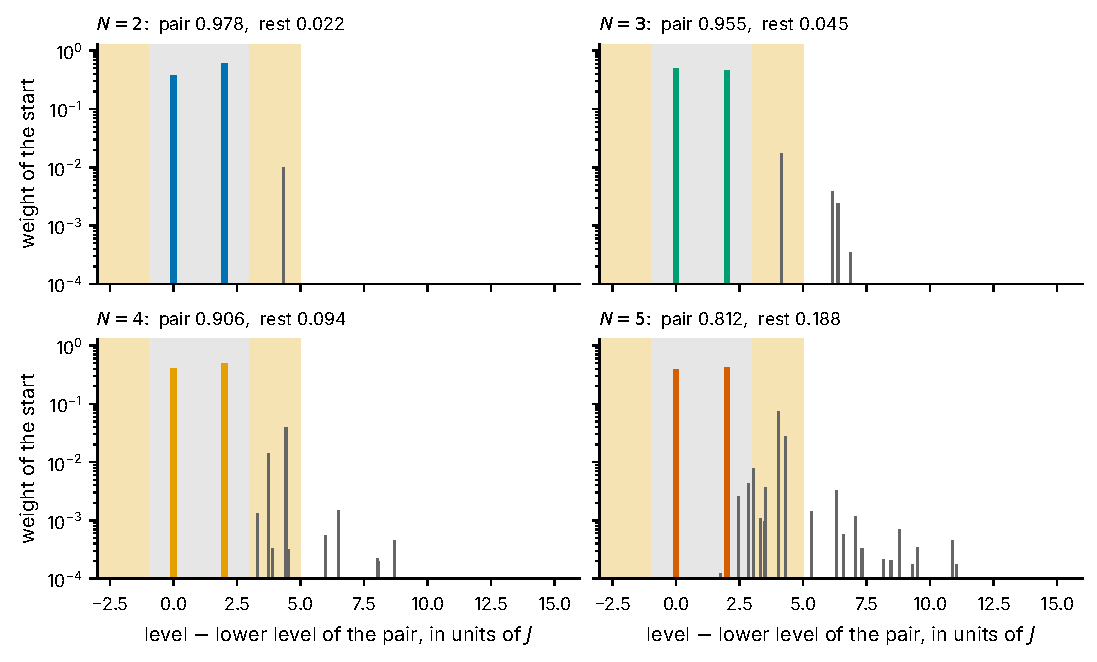
\includegraphics[width=0.8\textwidth]{figures/fig_spectrum.pdf}
\caption{\textbf{The correlated start in the eigenbasis of $\hat H$} at the resonance tilt, $k=20$ modes per particle. Each line is one eigenlevel; its height is the weight of the start on it, on a logarithmic axis; the horizontal axis is the distance from the lower level of the pair in units of $J$. Colour: the pair. Shading: within $J$ of either level of the pair (grey) and $1$--$3J$ from it (orange). The title of each panel gives the weight of the pair and of the rest; at $N=4,5$ part of the rest sits on levels not computed (Fig.~\ref{fig:dressing}b).}
\label{fig:spectrum}
\end{figure}

Table~\ref{tab:static} and Fig.~\ref{fig:spectrum} show that for $N=2,\dots,5$ the start lies on two eigenstates and a thin cloud of others: the symmetric and antisymmetric combinations of the all-left cluster (all particles in the crowded valley) and of the cluster with particle $0$ moved to the other valley. Their splitting $2J$ is the frequency of the main oscillation. The weight of the pair falls with $N$ at fixed basis size and rises with $k$ (Fig.~\ref{fig:dressing}a); it converges at $N=4$ but not at $N=5$, and no $N=6$ spectrum is converged. The small-basis values at $N=4$ ($k=12$) are a basis artefact.

\begin{figure}[ht]
\centering
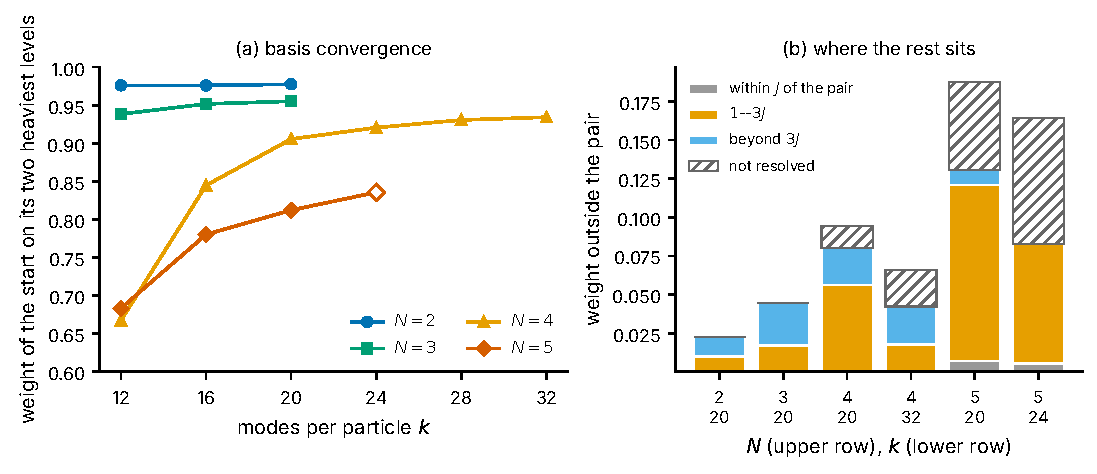
\includegraphics[width=0.8\textwidth]{figures/fig_dressing.pdf}
\caption{\textbf{The pair and the dressing.} (a) Weight of the start on the pair against the number of modes per particle $k$ (lines, $N=2$--$5$). The open symbol is a Lanczos list that resolves only part of the weight (Table~\ref{tab:start}). The $N=4$ curve converges; the $N=5$ curve has not. (b) The weight outside the pair, split by the distance to the nearer level of the pair: within $J$ (grey), $1$--$3J$ (orange), beyond $3J$ (blue), and weight not on any computed level (hatched). Upper axis label: $N$; lower: $k$. At $k=12$ a large part of the rest sits within $J$ of the pair at $N=4,5$; that part is a basis artefact (it vanishes for $k\ge16$) and is not shown.}
\label{fig:dressing}
\end{figure}

The weight outside the pair (Fig.~\ref{fig:dressing}b) is small far from the pair and about the same for all $N$; the part that grows with $N$ sits at $1$--$3J$, on internal levels softer than the transfer itself. This is the dressing of the transfer by soft internal motion of the cluster, and it is the quantity on which the scaling of the problem depends (Section~\ref{sec:openproblem}). It does not fall when the barrier is raised, although $J$ does (Table~\ref{tab:Ascan}).

\subsection{One transfer channel and an exact symmetry}
\label{sec:parity}

The pair is a closed two-state system at $N\le4$ for three structural reasons (Fig.~\ref{fig:parity} and Table~\ref{tab:levels}, Appendix~\ref{app:static}). The reflection $y_i\to-y_i$ of all particles is an exact symmetry of $\hat H$ and $\Op$; the start is even, so the odd levels, including those between the two members of the pair, carry no weight. The transfer of more than one particle is far from the pair (\emph{sector exclusion}). And because particles are distinguishable, the states in which another particle moves instead of particle $0$ lie a few $J$ from the pair (\emph{label fragmentation}); that margin is why the offsets $C_0$ matter (Appendix~\ref{app:choice}), it is not large, and it is not known to survive for $N\gtrsim6$.

\subsection{Most of the entropy is static}
\label{sec:static-entropy}

\begin{figure}[htpb]
\centering
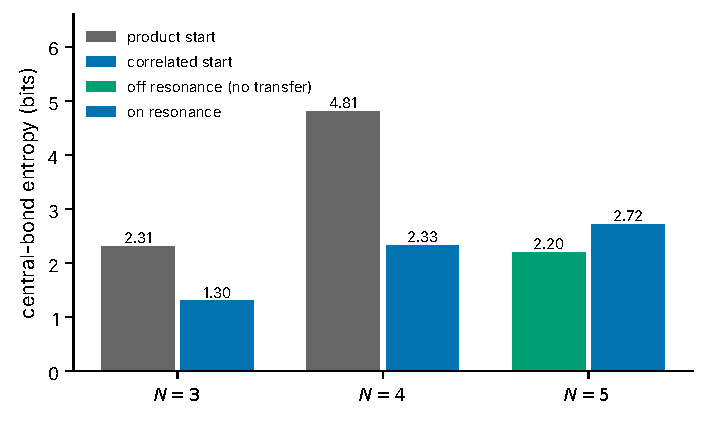
\includegraphics[width=0.5\textwidth]{figures/fig_control.pdf}
\caption{\textbf{How much of the central-bond entropy is already there before anything moves.} Left and middle: the product start (a quench that ignores the correlation hole of particles sharing a valley) against the correlated start. Right, $N=5$: the same start off resonance, where the cluster stays in one isomer, against the resonant run. The off-resonance entropy is $\num{off_diff}$ bit below the resonant one.}
\label{fig:control}
\end{figure}

Away from resonance the cluster stays in one isomer and no tunneling takes place, yet the central-bond entropy keeps most of its resonant value (Table~\ref{tab:control}, Fig.~\ref{fig:control}). Together with the closed two-state structure this changes the reading of Section~\ref{sec:measured}: those entropies are, for the most part, the static entanglement of the correlated isomers, namely the correlation hole of particles that share a valley, which the correlated start carries from $t=0$. In the ideal case in which the start is exactly a superposition $a|F\rangle+\sum_ib_i|I_i\rangle$ of a product state $|F\rangle$ and states with one particle moved, every cut has Schmidt rank at most two, so the entropy added by the transfer is at most one bit for any $N$ (Proposition~\ref{prop:cond}). Matrix-product-state cost curves built on the entropy of the evolved state price the isomers; they do not by themselves show that the dynamics is hard.

\begin{table}[ht]
\centering
\small
\caption{The control without tunneling: $N=5$, $k=12$, correlated start, away from resonance ($c=\num{off_c}$, the start stays in one isomer) against the resonant run (Fig.~\ref{fig:control}). Same window $T=\num{off_T}$\num{off_lb}.\num{off_note}}
\label{tab:control}
\begin{tabular}{lrr}
\toprule
 & off resonance & resonance \\
\midrule
lowest value of $\langle\Op\rangle/\langle\Op\rangle(0)$ & 0.75 & 0.27 \\
central bond $\Snat$ & 2.20 & 2.72 \\
mean one-particle entropy $\bar S_1$ & 1.60 & 1.88 \\
edge weights $w_{ij}$ (range) & 0.44--1.15 & 0.92--1.16 \\
largest graph excess over the exact entropy & 0.30 & 0.48$^\dagger$ \\
rank correlation, graph against exact orders & 0.87 & 0.46 \\
time of the central-bond maximum & 144 & 197 \\
\bottomrule
\end{tabular}
\par\smallskip\footnotesize $^\dagger$ largest over all $N\le6$ (Fig.~\ref{fig:entropy}a), not for $N=5$ alone.
\end{table}


\subsection{A conditional reduction and the number of cosines}
\label{sec:cond}

\begin{cprop}\label{prop:cond}\stC{}
Let $|F\rangle$ be the correlated all-left state and $|I_0\rangle$ the correlated state with particle $0$ on the right. Suppose that for $0\le t\le\Tobs$ the evolved state stays, up to an amplitude error $\delta$, in the span $\mathcal S$ of $|F\rangle$, $|I_0\rangle$ and $M$ further eigenstates $|s_1\rangle,\dots,|s_M\rangle$ of $\hat H$ (the sidebands). Then
\[
f(t)=\sum_{m,n}c_m^\ast c_n\,O_{mn}\,e^{i(E_m-E_n)t}+O(N\delta),\qquad m,n\in\{1,\dots,M+2\},
\]
is a sum of at most $(M+2)(M+3)/2$ cosines whose frequencies, weights and amplitudes are static quantities of $\hat H$. In the ideal case $M=0$, with product states of left and right orbitals and any number of labelled states with at most one particle on the right, every particle cut has Schmidt rank at most two and entropy at most one bit for any $N$. For correlated states of bond dimension at most $\chi_0$ in a common ordering, the bond dimension of the state is at most $(M+2)\chi_0$ at all times.
\end{cprop}

The first statement is a finite-dimensional superposition, and the rank bounds follow because $a|F\rangle+\sum_ib_i|I_i\rangle$ is a sum of two product vectors across any cut (proof in Appendix~\ref{app:proofs}). What is not elementary is whether $M$ stays small and whether the static inputs are cheap.

\begin{figure}[htpb]
\centering
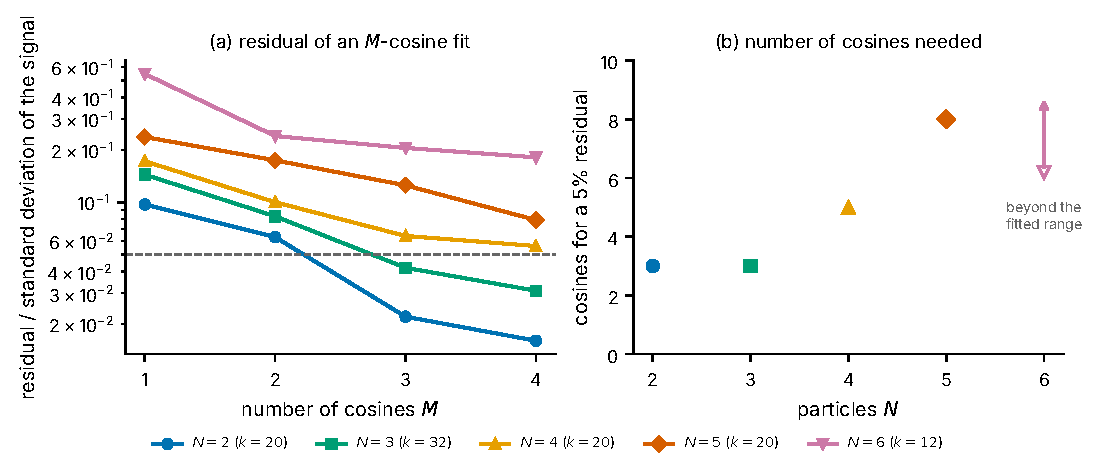
\includegraphics[width=0.8\textwidth]{figures/fig_cosines.pdf}
\caption{\textbf{How many cosines the signal needs.} (a) Residual of a free fit of $M$ cosines to $\langle\Op\rangle(t)$ on the stored time series ($T=\num{Tprot}$), in units of the standard deviation of the signal, for the largest basis size available at each $N$. (b) The number of cosines for a residual of $5\%$; the open symbol at $N=6$ marks that no fit with up to eight cosines reached it (one run, $k=12$, not converged). The fit chooses its frequencies freely; it is a measure of the structure of the signal, not a prediction from static energies.}
\label{fig:cosines}
\end{figure}

A few cosines do explain the signal at $N=2,3$, but the number needed for a given residual grows with $N$ (Table~\ref{tab:mc}, Table~\ref{tab:static}, Fig.~\ref{fig:cosines}b), the same trend as the dressing seen in the time domain. This cannot say whether the growth continues, and it does not by itself decide the cost of the task, since obtaining $M$ frequencies and weights is a static problem.

\subsection{Where the regime ends}
\label{sec:regimeend}

\begin{figure}[htpb]
\centering
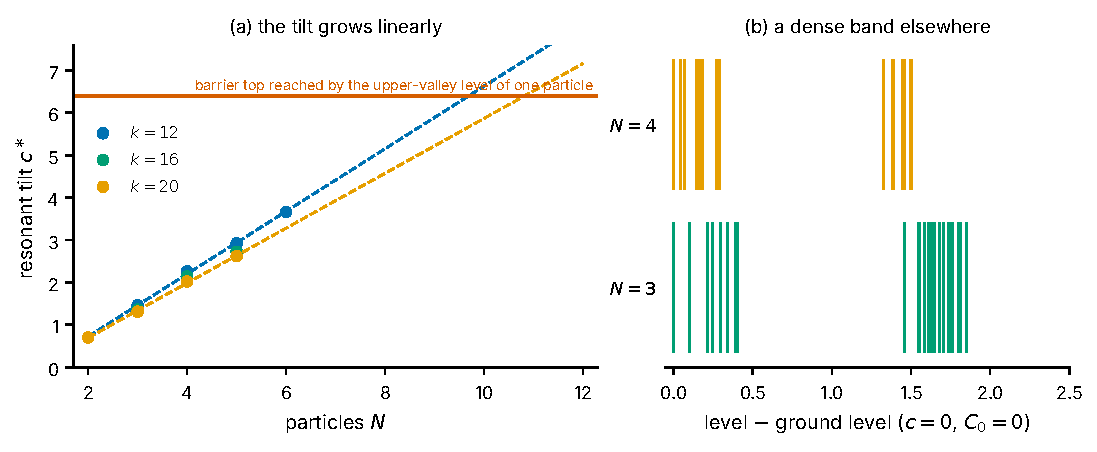
\includegraphics[width=0.8\textwidth]{figures/fig_tilt.pdf}
\caption{\textbf{The resonance tilt and the end of the regime.} (a) The tilt $c^\ast$ at which the all-left and one-moved clusters are degenerate, against $N$, for three basis sizes; it rises by about $\num{fu_cstep_lo_k12}$--$\num{fu_cstep_hi_k12}$ per particle at $k=12$, nearly linearly. Dashed lines extend the straight lines through the measured points. The horizontal line is the tilt at which the lowest level localized in the raised valley of the one-particle tilted well reaches the top of the barrier ($c=\num{fu_ctop}$; finite differences, a rough one-body picture). (b) With a symmetric trap and no tilt or offsets ($c=0$, $C_0=0$) the lowest levels form a dense band with a gap above it: a different task from the tilted transfer.}
\label{fig:tilt}
\end{figure}

The resonant tilt rises nearly linearly with $N$ and shows no bending through the measured sizes (Fig.~\ref{fig:tilt}a). In the one-particle picture of the tilted well the upper-valley level reaches the top of the barrier at a tilt that the straight lines reach at $N\approx\num{fu_Ntop_lo}$--\num{fu_Ntop_hi}. The entropy extrapolations of Section~\ref{sec:larger} cross this point, and whether the transfer continues as a many-body process past it is open. A trap depth that grows with $N$ is a different family: the rule must be fixed in advance, and the classical and quantum costs recomputed. With a symmetric trap and no tilt (Fig.~\ref{fig:tilt}b) the lowest band is a dense many-occupation manifold with permutation multiplets, a different task that was not simulated in time.

\subsection{The open problem}
\label{sec:openproblem}

The cost of the task, as defined, is the cost of the static \emph{dressed-transfer spectrum}: the number $M(N)$ of sidebands needed for error $\varepsilon N$, and the cost of their energies, weights and matrix elements. If the dressing is harmonic (a displaced, Duschinsky-mixed oscillator bath) the problem is a spin--boson problem, which is heuristically easy classically. If it is strongly anharmonic with soft modes comparable to $J$, no classical method with a known polynomial cost applies. Sign-free structure (distinguishable particles) makes imaginary-time and instanton methods applicable (Section~\ref{sec:mc}), but neither a polynomial bound nor a hardness proof is known. The measurements say only that the weight outside the pair grows with $N$ at fixed basis size, that the growing part sits at $1$--$3J$, and that $J$ is not small compared with it at $N=4,5$.

\paragraph{Hardness is unprovable for this fixed family.} The observable is a function of positions, so its time derivative is bounded by a constant times $N$ and $f$ can be tabulated to the allowed error on a finite set of points for every $N$ (Appendix~\ref{app:static}). The table exists but is not an algorithm (a non-uniform statement), so no reduction-based hardness result is possible for the task as defined. Statements can only concern the scaling of the best known methods, or a different family with free instance parameters.

\paragraph{What is not established.}
\begin{itemize}[itemsep=0.15em]
\item The dressing series has few points at basis sizes that are still moving at $N=5$ (Table~\ref{tab:start}); extrapolating it to $N=6,7$ is not a measurement.
\item Gaussianity of the dressing is undecided: the test is the harmonic (Huang--Rhys) prediction of $B_2$ from the two constrained isomers against the measured $B_2$ at $k\ge16$, and it was not run.
\item $N=6$ and the basis convergence at $N=5$ are unfinished; everything in this section is for $N\le5$ unless stated.
\item The cosine counts are free fits to one stored signal per case, not predictions.
\item No claim is made that a classical method reproduces the signal at large $N$, nor that none does.
\end{itemize}

\FloatBarrier
